\chapter{Tactile Reactive Control Strategy}\label{IROS2019}

This chapter outlines an experiment which tests and compares the performance of two approaches to grasping a moving object. This experiment specifically evaluates the tolerance for temporal and spacial errors for two different grasping strategies. The first approach (typical in the prior art) is a vision-only approach. Image sensors localise and track a target object as it moves, and open-loop control is used to close the gripper when the object is within a defined range. This approach acts as the control group to which the second approach is compared.

The second approach evaluated in this experiment explores if a performance improvement can be made by supplementing the vision system with tactile feedback from the gripper. The grasp reacts to feedback from tactile sensors located in the gripper (i.e. the motion of the gripper closing is dependant on how the object makes contact with it). If such a strategy was successful in increasing the tolerance for error, both temporal and spacial, in the estimate of an appropriate interception point along the target objects trajectory the computational overhead associated with grasping moving objects would be reduced. Since estimations can be less accurate and still result in a successful grasp. Furthermore, the need to place sensors in the environment to accurately track the target object's trajectory is removed and the problem can be tackled with on-board sensors. This allows such a solution to be deployed on a general purpose, mobile, service robot which cannot rely on an existing infrastructure of sensors and does not have vast quantities of computing power. 

\section{Reactive Strategy}\label{subsec:strategy}

The reactive tactile grasping is a novel approach, proposed in this research, and as such, needs to be tested and compared to the traditional approach prior to any further optimisation of the contribution of tactile feedback. Thus, such optimisations are outside the scope of this experiment and chapter but are address later in this document. The grasping strategy used in this research was based on three basic rules:

\begin{enumerate}
    \item The grasp is triggered when the object first makes contact with the gripper (see Figs. \ref{subfigure:Stage1} \& \ref{subfigure:Stage2}). This contrasts to the vision-only system which would close at the estimated interception time.
    \item The gripper attempts to reduce the spacial error by adjusting its position in the x-axis. Tactile sensors detect the point of contact and trigger the gripper to move along the x-axis accordingly . This is represented by arrow 1 in Fig. \ref{subfigure:Stage3}
    \item The finger which comes into contact with the object first delays its closing motion while the other finger begins to close, resulting in the grasp being slightly asymmetric as seen in Fig. \ref{subfigure:Stage4}. The vision-only system lacks the information about the contact point(s), preventing the grasping motion from being adapted to the object position. This is represented by arrow 2 in Fig. \ref{subfigure:Stage3}
\end{enumerate}

\begin{figure}[ht]
    \centering
    \begin{subfigure}{.45\linewidth}
        \centering
        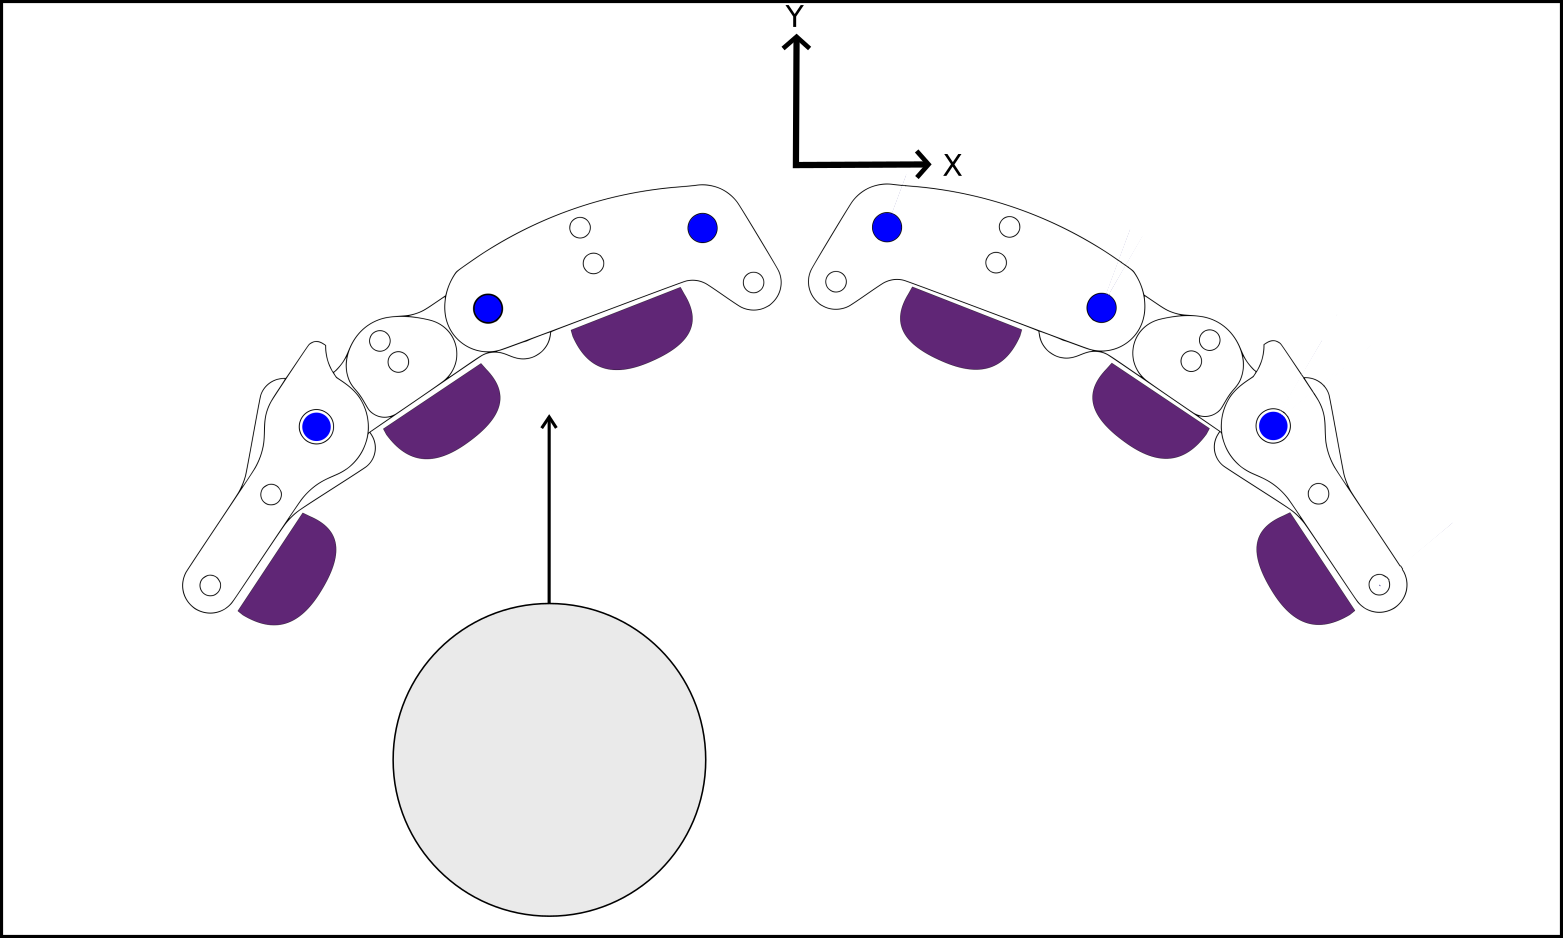
\includegraphics[width=0.9\textwidth]{Images/stage1.png}
%  
\includegraphics[width=.4\textwidth]{Images/placeholder.png}
        \caption{Stage 1}
        \label{subfigure:Stage1}
    \end{subfigure}
    \begin{subfigure}{.45\linewidth}
        \centering
        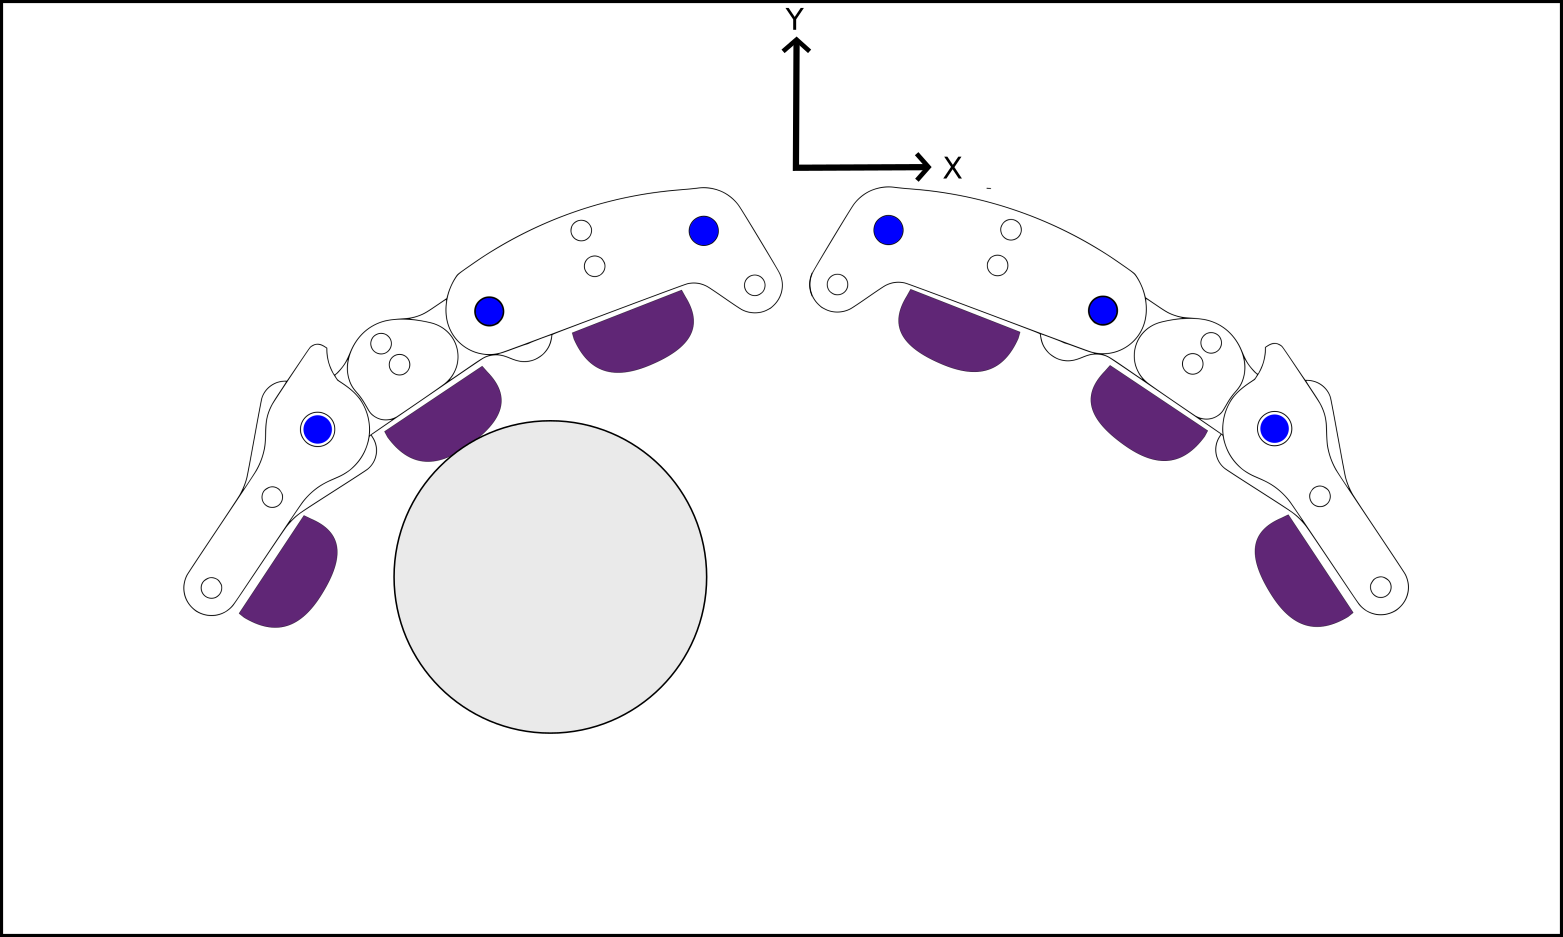
\includegraphics[width=0.9\textwidth]{Images/stage2.png}
%    
\includegraphics[width=.4\textwidth]{Images/placeholder.png}
       \caption{Stage 2}
        \label{subfigure:Stage2}
    \end{subfigure}
    \begin{subfigure}{.45\linewidth}
        \centering
        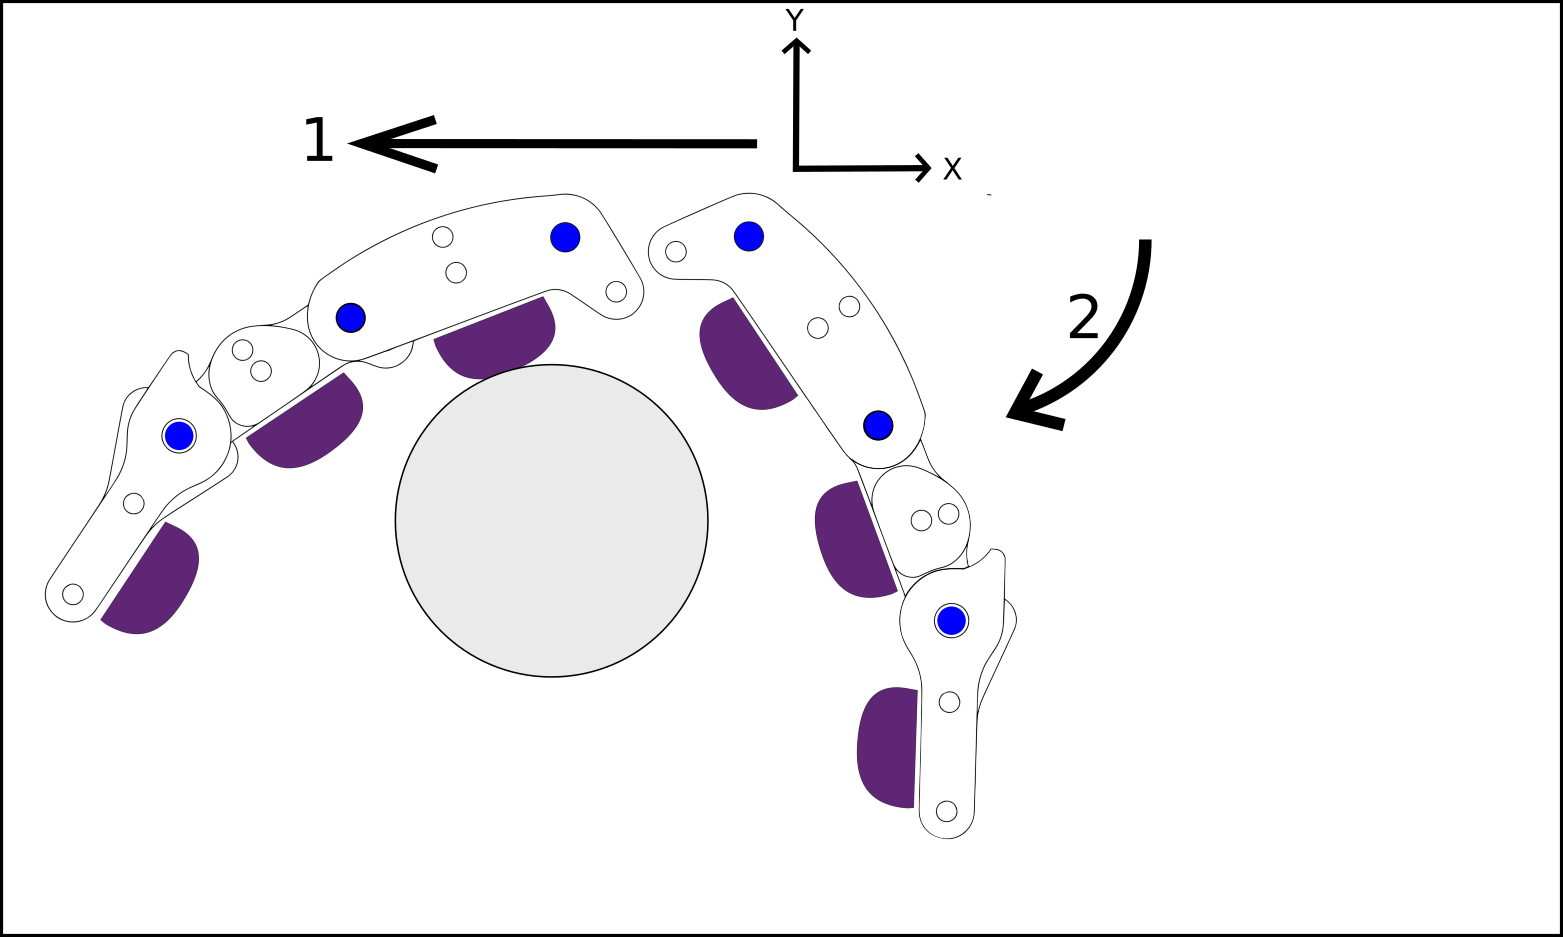
\includegraphics[width=0.9\textwidth]{Images/stage3.png}
%    
\includegraphics[width=.4\textwidth]{Images/placeholder.png}
        \caption{Stage3}
        \label{subfigure:Stage3}
    \end{subfigure}
    \begin{subfigure}{.45\linewidth}
        \centering
%    
\includegraphics[width=.4\textwidth]{Images/placeholder.png}
    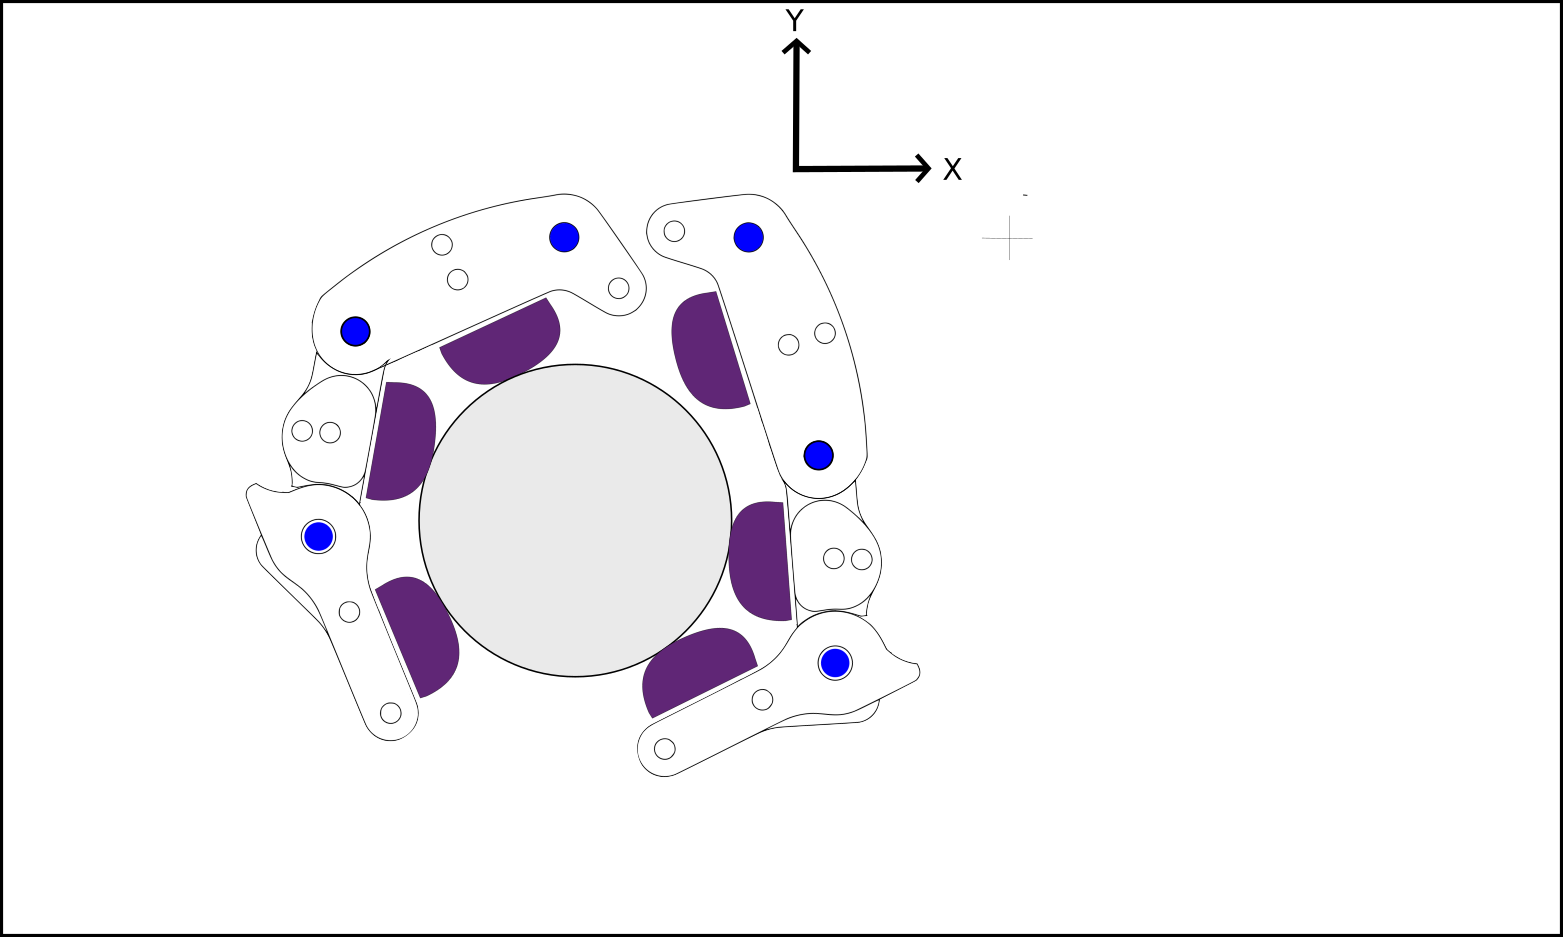
\includegraphics[width=0.9\textwidth]{Images/stage4.png}
        \caption{Stage 4}
        \label{subfigure:Stage4}
    \end{subfigure}
    \caption{Illustration of the simple tactile enabled, reactive grasping strategy: (a) Stage 1: Ball approaches gripper with a negative spacial offset in x,(b) Stage 2: Ball makes contact with gripper, a tactile sensor in the left finger triggers the grasp,(c) Stage 3: Gripper attempts to grasp the ball, its strategy is informed by tactile sensing,(d) Stage 4: Grasp is successful}
\label{fig:Tactile Stragety}
\end{figure}

\subsection{Experimental Setup}

The experiment involved the use of a two finger (each with 3 degrees of freedom) pincer gripper, outlined in Chapter \ref{Chapter:GripperDesign}, which was tasked with grasping a moving billiards ball. The grasper is actuated using servo motors controlled by an ESP32. Similarly the grasping strategy, outlined above, is implemented using the same ESP32 micro controller \cite{gitIROS}. The grasping unit was actuated in the x-direction (Fig. \ref{fig:Tactile Stragety}) along a linear rail using a servo motor. Each finger contained three tactile sensors, one on each flange, these tactile sensors are outlined in Chapter \ref{Chapter:TactileSensing}.

\begin{figure}[ht]
    \centering
    \begin{subfigure}{.8\linewidth}
        \centering
        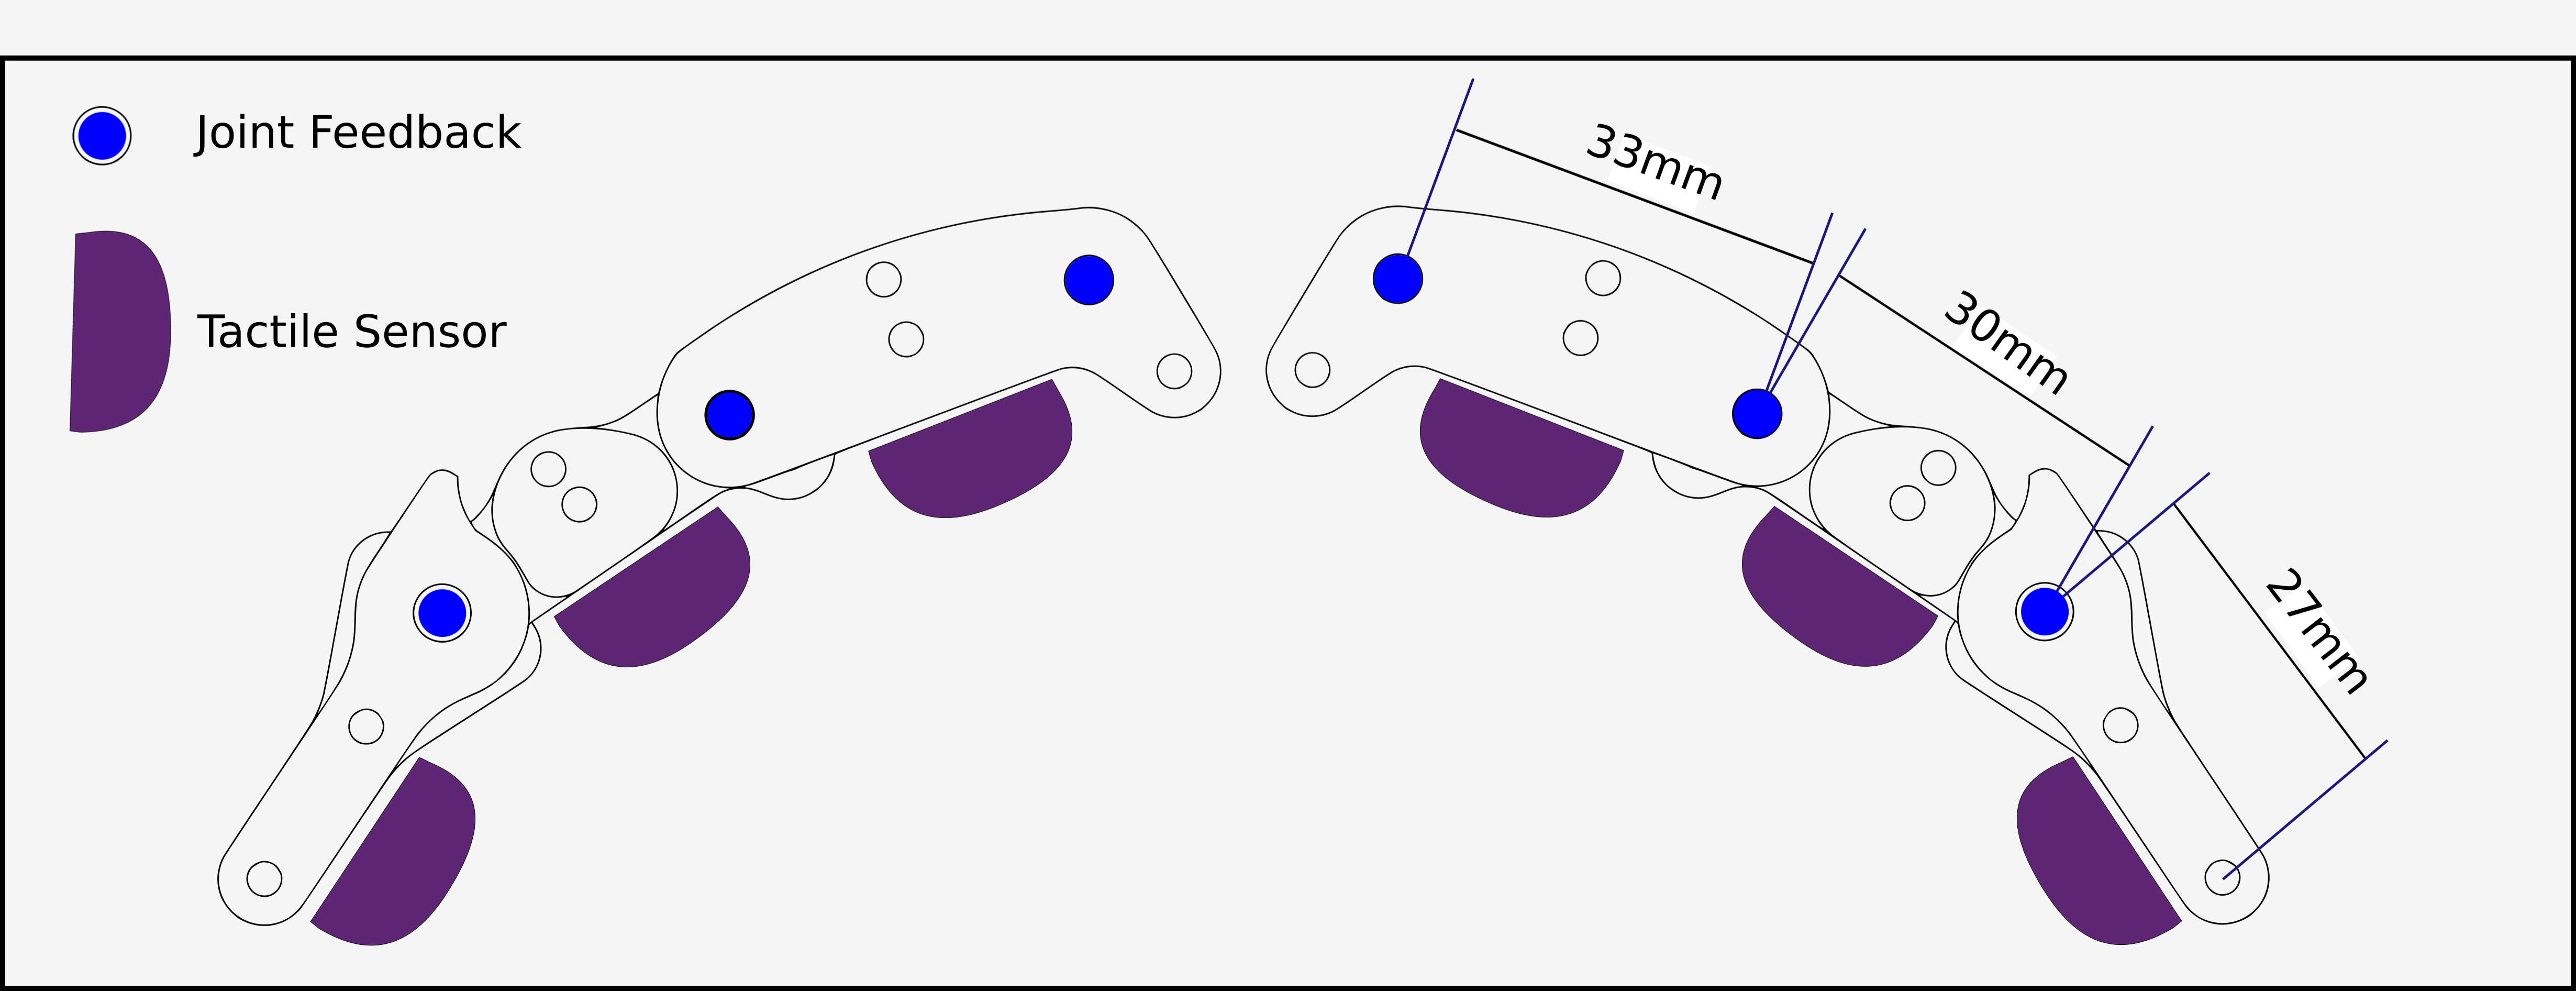
\includegraphics[width=\textwidth]{Images/Dimensions.png}
%        
\includegraphics[width=.4\textwidth]{Images/placeholder.png}
        \caption{Drawing of pincer gripper with dimensions}
        \label{subfig:1a}
    \end{subfigure}
    \begin{subfigure}{.8\linewidth}
        \centering
    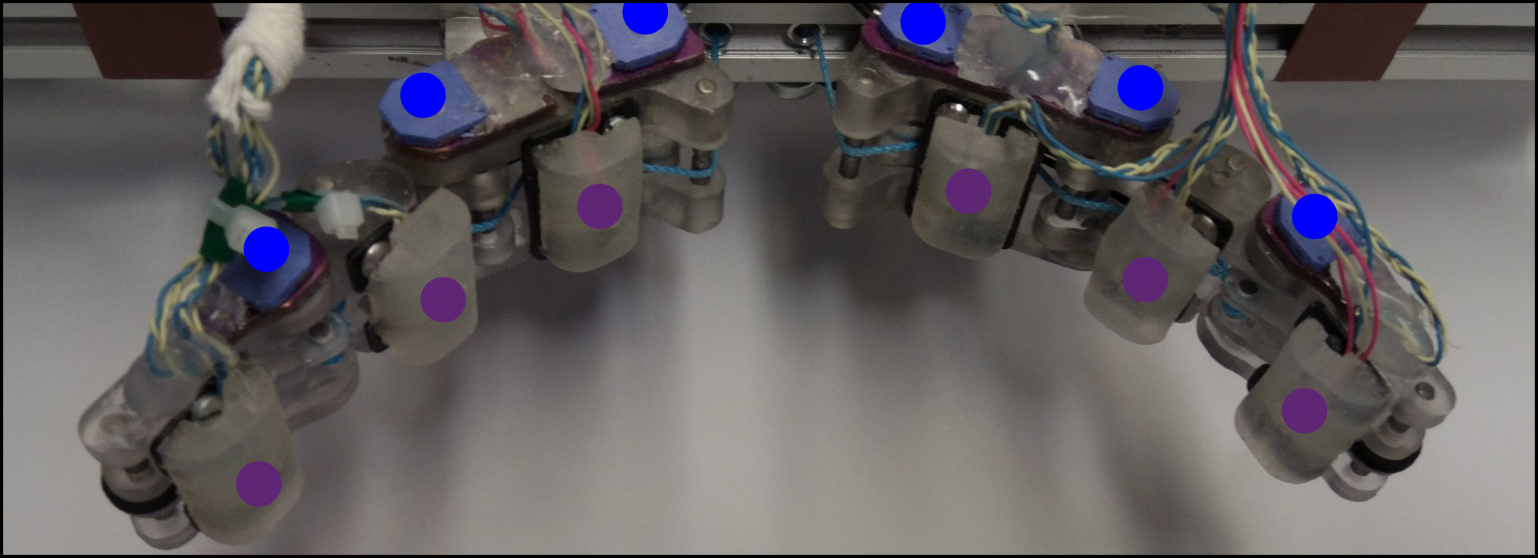
\includegraphics[width=\textwidth]{Images/LabeledPhoto.png}
%    
\includegraphics[width=.4\textwidth]{Images/placeholder.png}
       \caption{Photograph of pincer gripper used}
        \label{subfig:1b}
    \end{subfigure}
 \caption{Under-actuated, two finger, pincer gripper with distributed tactile sensing, a soft compliant covering, and joint position feedback.}
\label{fig:Gripper}
\end{figure}

A spherically shaped object was used as the moving grasp object since it presents the same grasping problem regardless of orientation. The target object, a billiards ball, was chosen because of its properties, namely high stiffness, spherical shape, size, mass and confidence in it manufacturing quality.

The object was set in motion by rolling down an inclined plane, similar to the method outlined in \cite{DynamicObjectManipulation}. In this setup, a long bar of aluminium with a U profile was used to control the object's trajectory toward the gripper (in the negative z-direction according to Fig. \ref{subfigure:RigDiagram}). The ball was forced to maintain this trajectory until just before coming within the range of the gripper where is was  transitioned onto a horizontal planar surface. A photo and illustration of the control rig is given in figure \ref{fig:FullRig}. 

To ensure repeatability, the release of the ball was automated using servo motors. The speed of the ball was measured by monitoring the time the ball took to break two light gates, close to the gripper, placed at a known distance apart. The signals from the light gates were recorded by an independent system which used a logic analyser sampling at 2M samples/sec. Three different speeds were tested by releasing the ball from different heights on the inclined plane. The repeatability of this approach was validated prior to the experiment in a controlled tests (see Table \ref{tab:repeatability}).

As outlined in chapter \ref{Chapter:GripperDesign}, the simplification of the gripper to an under-actuated, two-fingered, pincer gripper and the grasping problem to a two dimensional case enabled the elimination of many variables which might have effected the repeatability of the experiment without relevance to the research question. This enabled a controlled experiment to be conducted where the effect of the embedded tactile sensing in the gripper can be isolated. Although simplified, this system is analogous to more complex manipulators used in other setups. 

\begin{figure}[ht]
    \centering
    \begin{subfigure}{.8\linewidth}
        \centering
        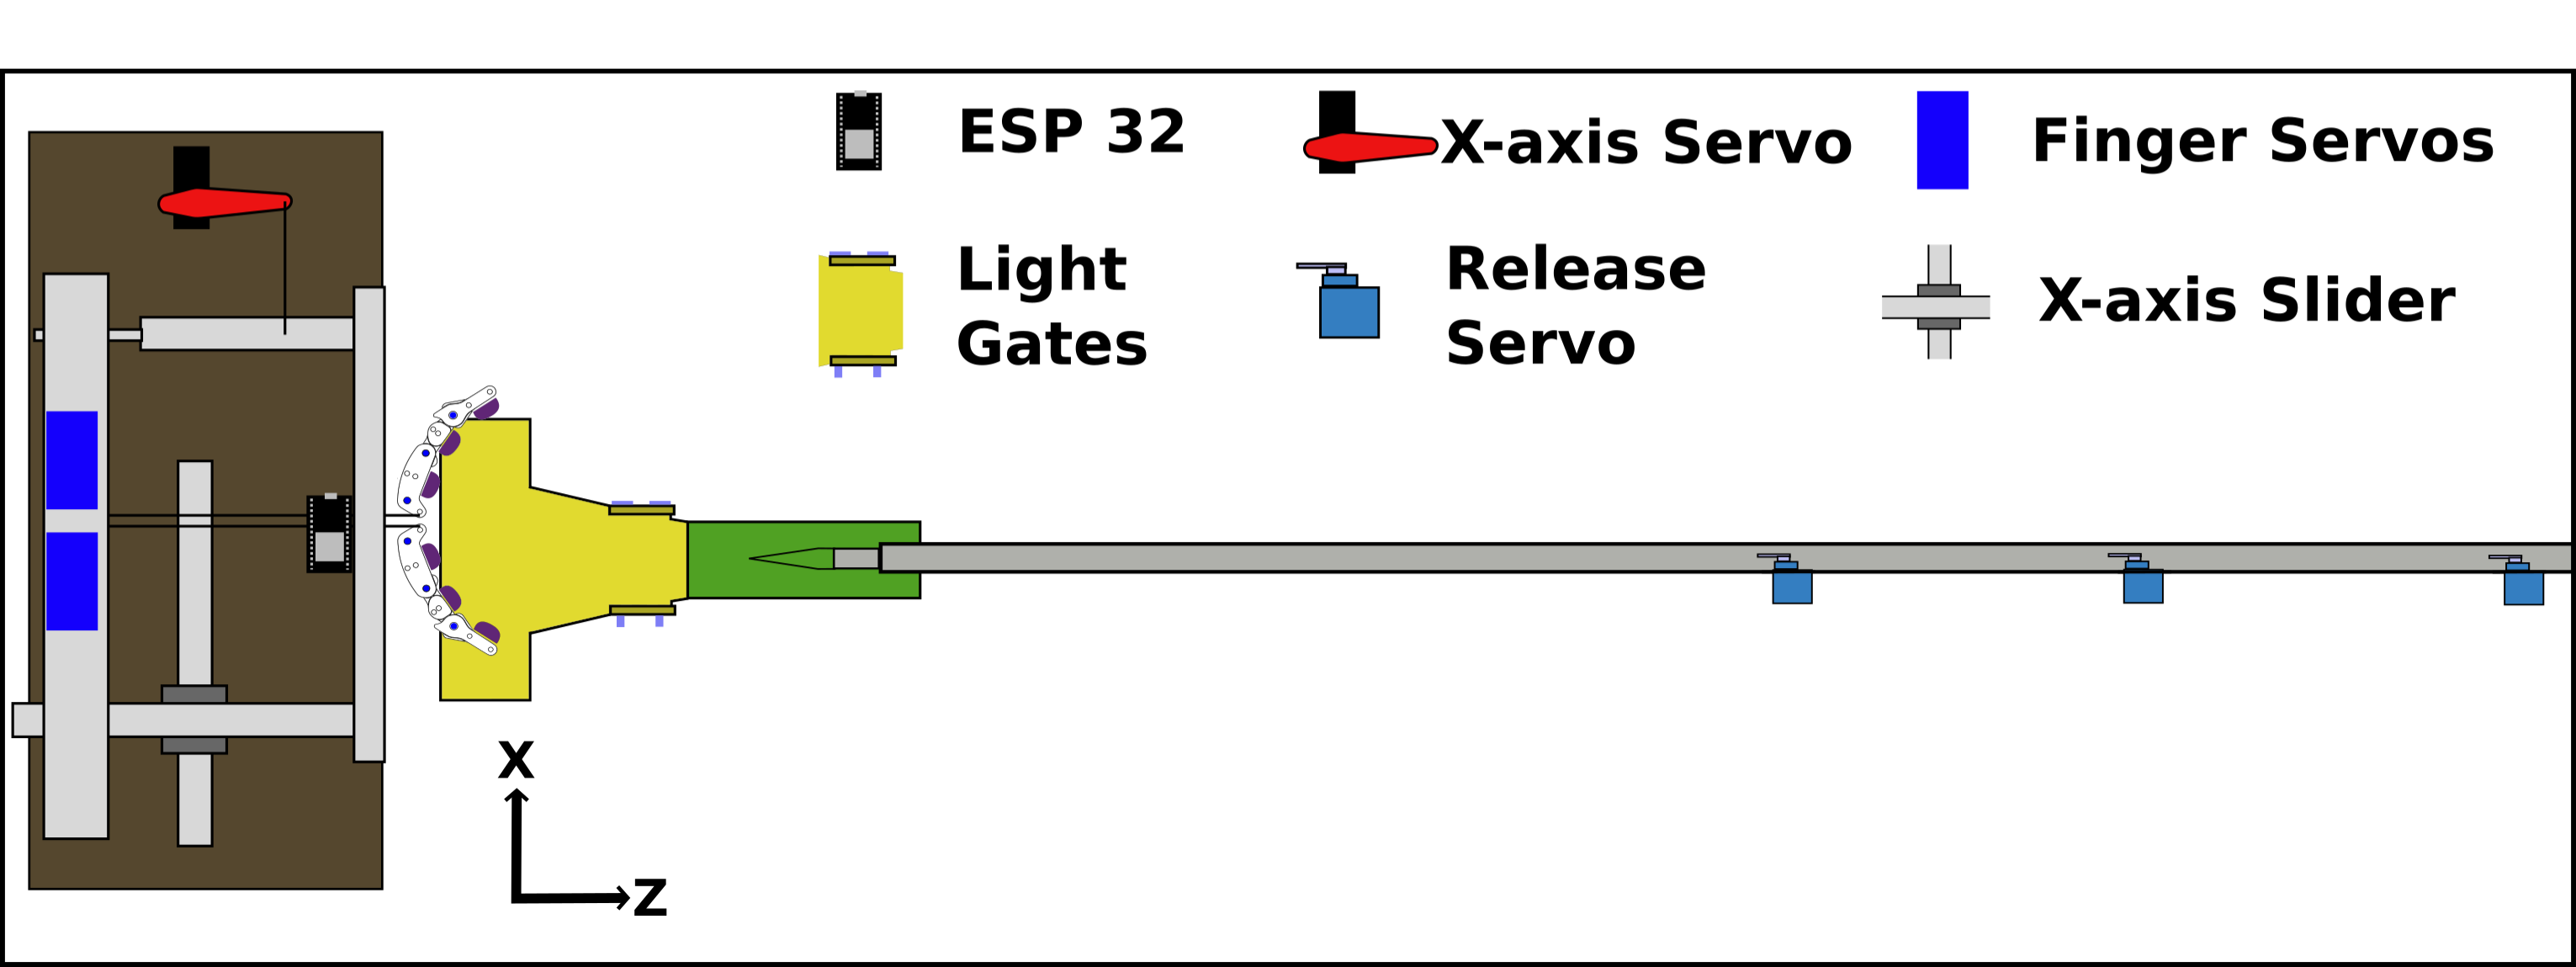
\includegraphics[width=\textwidth]{Images/FinalRig.png}
%        
\includegraphics[width=.4\textwidth]{Images/placeholder.png}
        \caption{}
        \label{subfigure:RigDiagram}
    \end{subfigure}
    \begin{subfigure}{.8\linewidth}
        \centering
    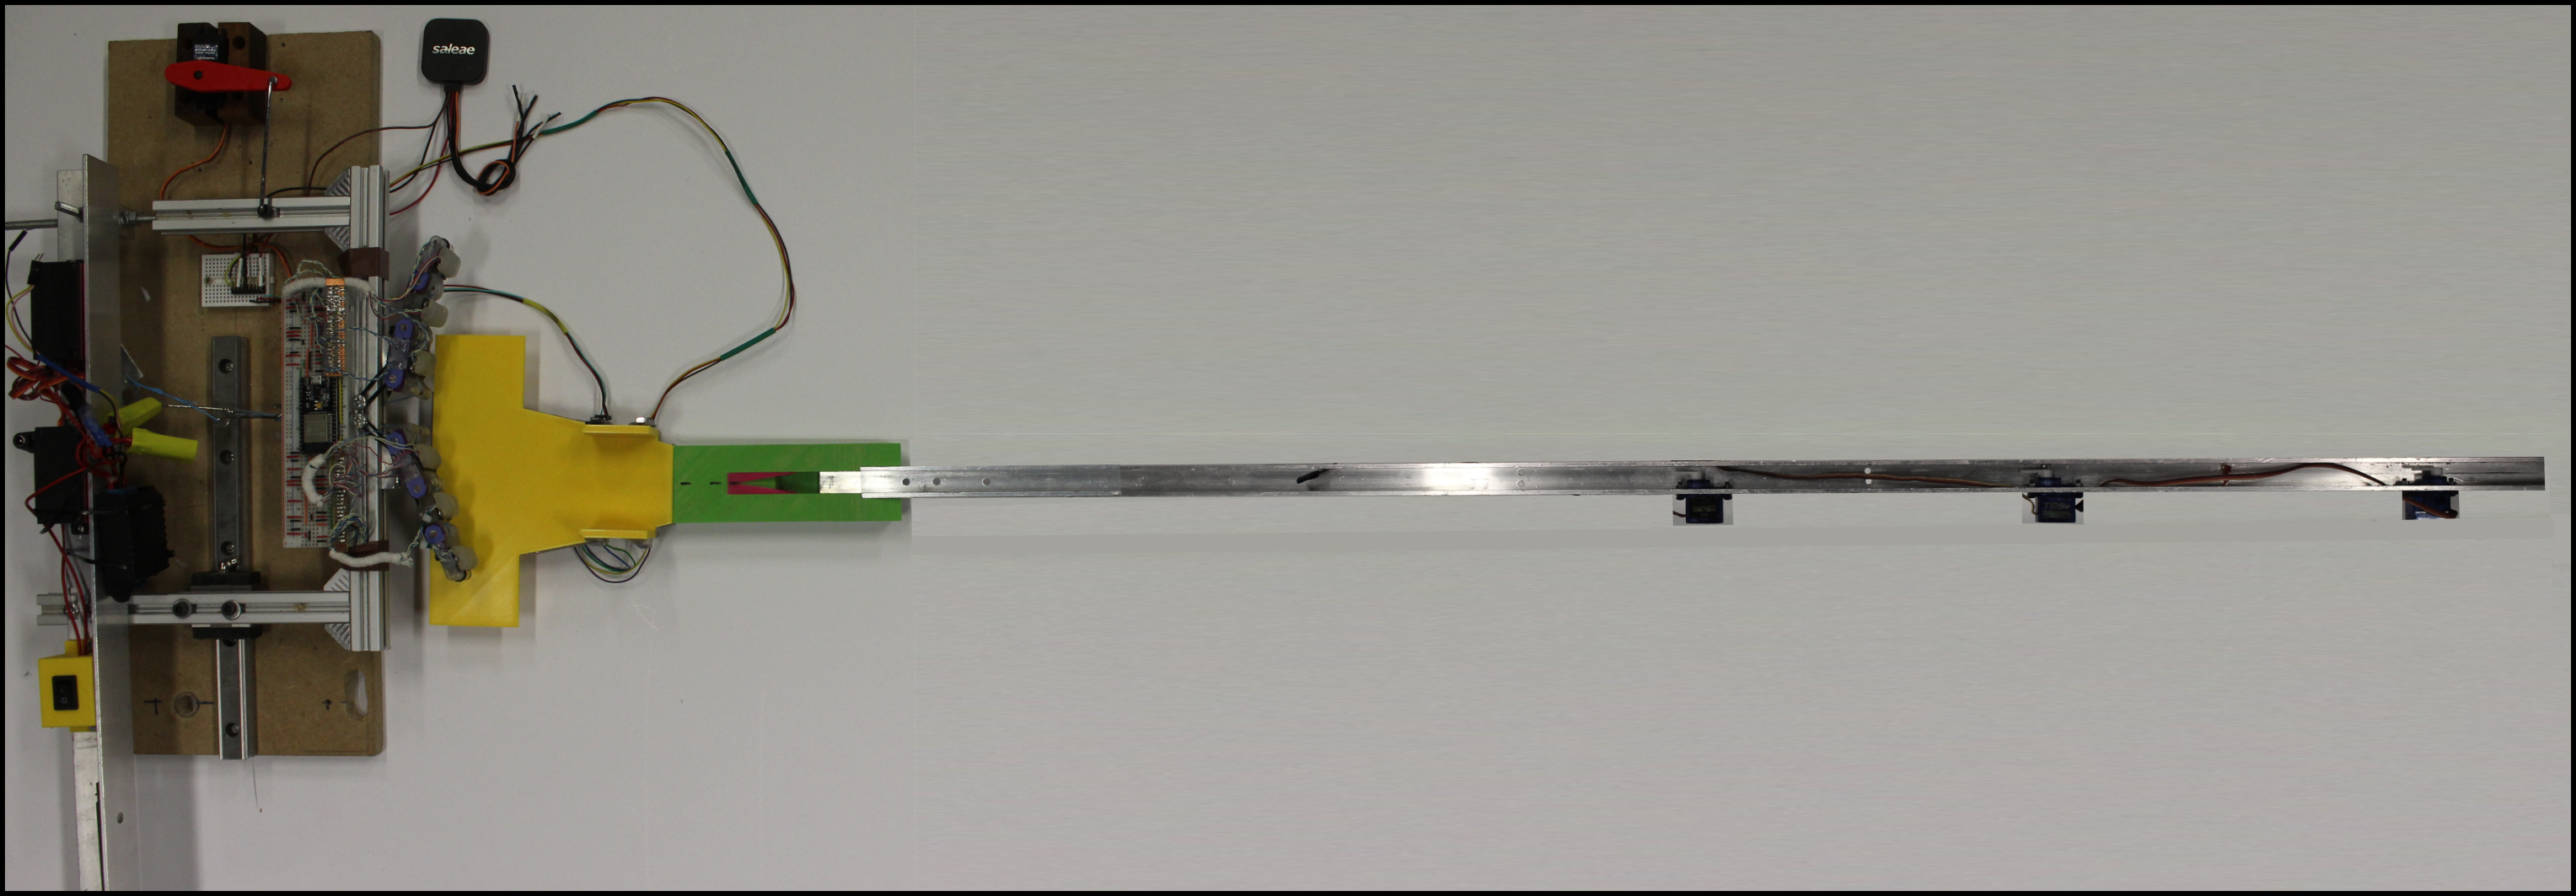
\includegraphics[width=\textwidth]{Images/RIG.png}
%    
\includegraphics[width=.4\textwidth]{Images/placeholder.png}
        \caption{}
        \label{subfigure:RigPhoto}
    \end{subfigure}
    \caption{Experimental Rig, a) diagram and b) overhead photo}
\label{fig:FullRig}
\end{figure}

\subsection{Experiment Design} % perhaps procedure
This research compares two approaches to grasping a moving object. The first was an analog of the vision-only approach where the light gates are used to inform grasp timing, but the grasp itself is achieved in an open-loop fashion. The second system used tactile sensing, implemented by following the rules outlined in section \ref{subsec:strategy}.

For each approach, the gripper's ability to successfully grasp the moving object was evaluated (dependent variable) for  different speeds (three levels), different offset distances (five levels) and different grasping strategies (four levels). Ten tests were conducted for each condition. 

The basic format of each test was the same. The ball would be placed on the ramp and held in place by one of the release servos. The servo would release the ball, allowing it to accelerate down the ramp. The ball was then transitioned to the flat plane where the gripper would attempt to grasp it. After the attempt, the platform on which the ball was rolling was lowered to remove any force, external to the gripper, from supporting the ball. The grasp was deemed a success if the gripper was able to support the full weight of the ball and a failure otherwise. 

\begin{table}[ht]
\centering
\begin{tabular}{r|c|c|c}
\textbf{(m/s)}           & \textbf{Speed 1}       & \textbf{Speed 2}       & \textbf{Speed 3}       \\
\hline
Mean                   & 0.82363 & 0.96363 & 1.08727   \\
Standard Deviation     & 0.01305 & 0.01252 & 0.02127   \\
Standard Error         & 0.00092 & 0.00089 & 0.00150   \\
%Confidence Level (95\%)       & 0.00182 & 0.00175 & 0.00297   \\
Number of Measurements & 200     & 200     & 200 
\end{tabular}
\caption{Speed data for 600 tests at 3 different speeds}
\label{tab:repeatability}
\end{table}

\section{Results}

Tests were conducted for three variations of the vision-only condition; each variation represented a different timing trigger from the point at which the ball passed the light gate. These timings (0ms, 5ms, 10ms) were determined empirically to represent fast, medium, and slower open-loop response conditions. In contrast, the test for the reactive grasping condition does not account for the three timings, since sensor stimulus triggers an near-instant response. The results across all of the test conditions are presented in Fig. \ref{fig:Results}, displaying the success rate under each set of conditions.

Analysis was performed to evaluate the influence of grasping strategy and spacial offset on grasp reliability across the range of object velocities. The success rates of the open-loop (OL) grasping strategy, for the three timings, and the reactive grasping strategy is shown in Fig. \ref{fig:meangraph}.

\begin{figure}[ht]
    \centering
    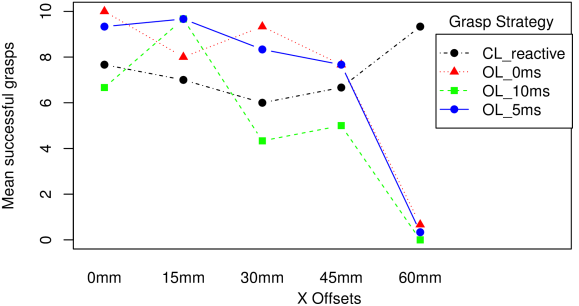
\includegraphics[width=0.475\textwidth]{Images/resultsgraph.png}
    \caption{Mean number of successful grasps per grasping strategy across all tests.}
    \label{fig:meangraph}
\end{figure}%

\begin{figure}[ht]
    \centering
    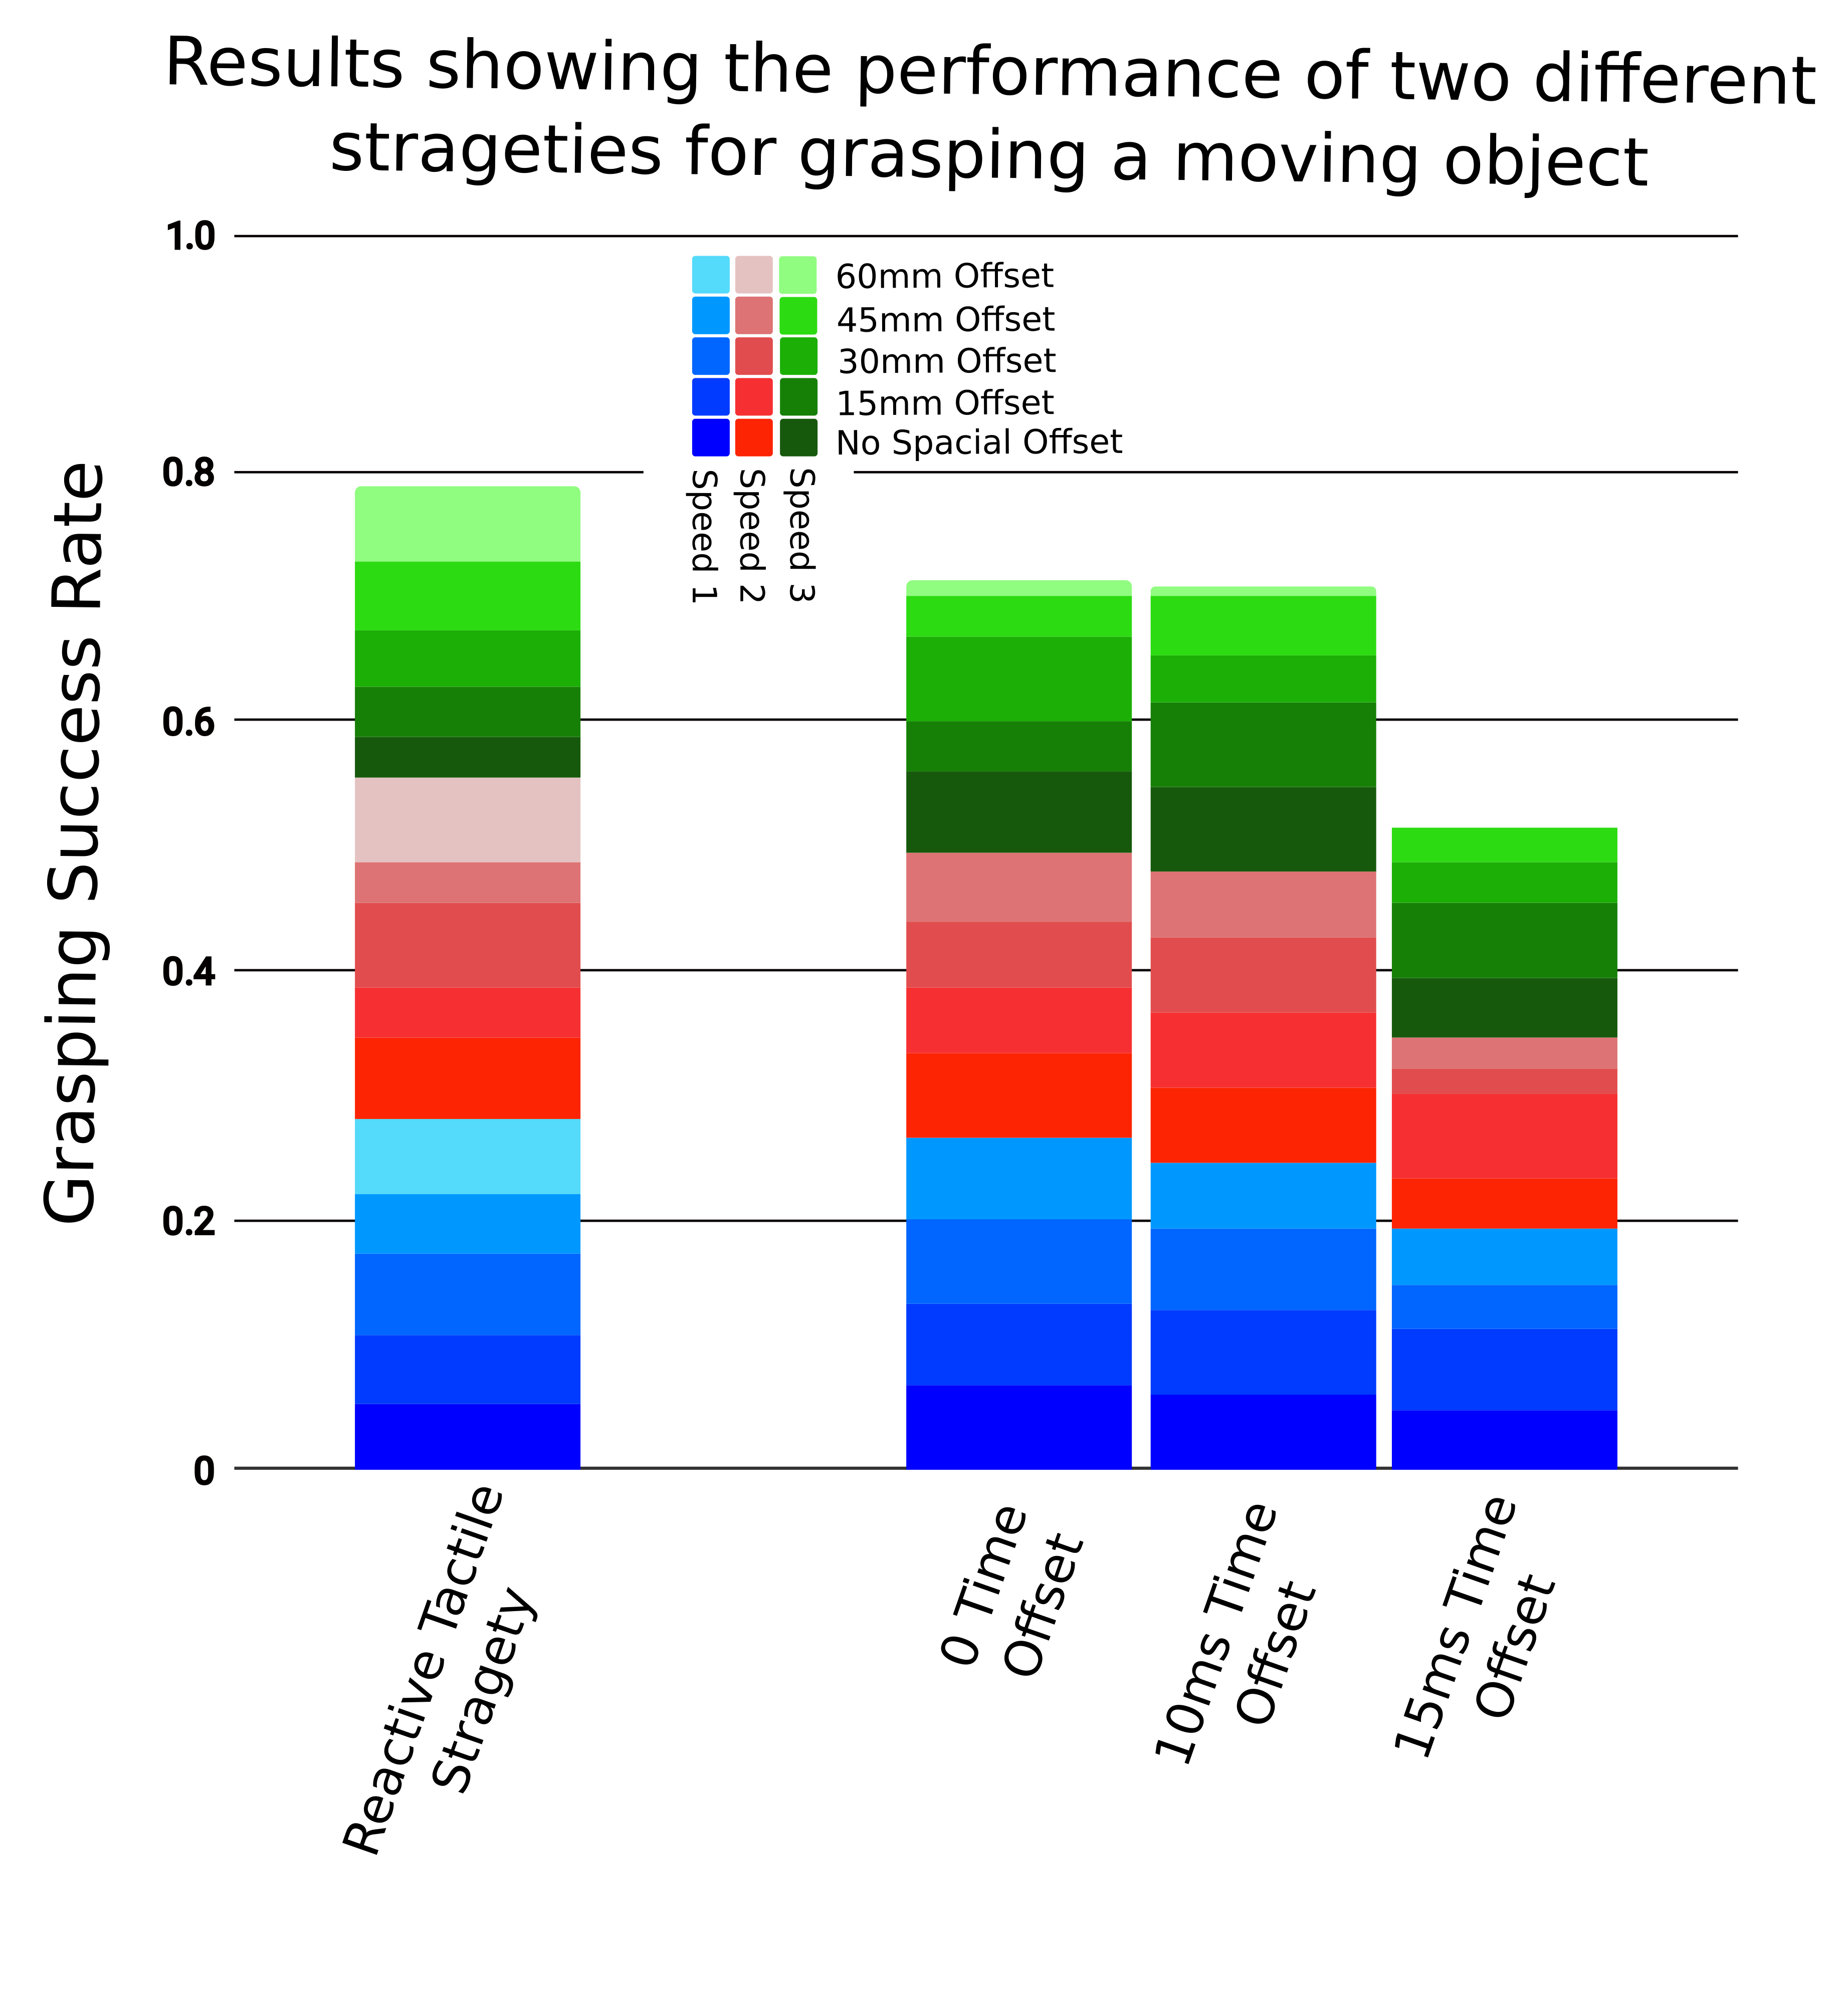
\includegraphics[width=0.9\textwidth]{Images/CrosslandResults.png}
    \caption{Representation of the grasping success rate based on stragety}
    \label{fig:CrosslandGraph}
\end{figure}%

\begin{figure}[ht]
    \centering
    \begin{subfigure}{.3\linewidth}
        \centering
        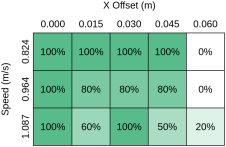
\includegraphics[width=\textwidth]{Images/VisionResults0.png}
%        
\includegraphics[width=.4\textwidth]{Images/placeholder.png}
        \caption{Time Offset 0ms}
        \label{subfigure:TimeOffset0ms}
    \end{subfigure}
    \begin{subfigure}{.3\linewidth}
        \centering
    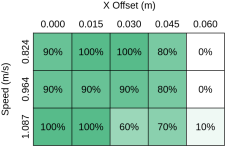
\includegraphics[width=\textwidth]{Images/VisionResults5.png}
%    
\includegraphics[width=.4\textwidth]{Images/placeholder.png}
        \caption{Time Offset 5ms}
        \label{subfigure:TimeOffset5ms}
    \end{subfigure}
    \begin{subfigure}{.3\linewidth}
        \centering
        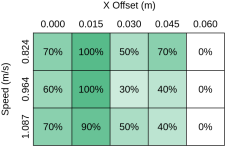
\includegraphics[width=\textwidth]{Images/VisionResults10.png}
%        
\includegraphics[width=.4\textwidth]{Images/placeholder.png}
        \caption{Time Offset 10ms}
        \label{subfigure:TimeOffset10ms}
    \end{subfigure}
    \hfill
    \begin{subfigure}{.3\linewidth}
        \centering
        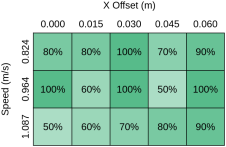
\includegraphics[width=\textwidth]{Images/Tactile.png}
%        
\includegraphics[width=.4\textwidth]{Images/placeholder.png}
        \caption{Tactile Sensing System}
        \label{subfigure:TactileSensingSystem}
    \end{subfigure}
    \caption{Successful grasp rates, observed over 10 tests under each set of conditions}
\label{fig:Results}
\end{figure}

The grasp reliability data was analyzed with a two-way factorial ANOVA. Significant (p $\leq$ 0.01) effects were found for the main effect of grasp strategy, F(3, 40) = 5.8049, p \textless 0.01 and grasp offset F(4, 40) = 25.8232, p \textless  0.01. A significant effect was also found for interaction between grasp strategy and positional offset, F(12, 40) = 7.0752, p \textless  0.01. A post hoc Tukey test, performed on the interaction effect, revealed significant differences at the highest offset value (i.e. spacial offset = 60mm) indicating that that the reactive grasping strategy outperformed each of the open loop strategies, p\textless0.01.

\section{Discussion}

% Speed has only a moderate effect on the visions systems ability to grasp while its effects are more pronounced for the tactile system due to inherient time error 
The results suggest that the vision-only system performs best at low spacial and temporal offsets. In this context, speed has a moderate effect on the grippers ability. In contrast, the effect of speed is greater for the reactive system. The grasping success rate is consistently poorer at higher speeds for this system. This highlights the importance of reaction time to this approach. The tactile strategy requires stimulus from contact between object and gripper to trigger the grasp whereas the vision-only system relies on an estimate interception time. However, the optimum grasp time is before contact between object and gripper. As a result, the tactile system has a small, inherent temporal offset from optimal. Therefore, the reduction in the time to react caused by a faster moving object, has a larger impact on the rate of successful grasping. 

%Temporal error can not grow
The first advantage offered by the tactile approach is observed when compared  to the visual system with a 10ms temporal offset. The tactile system significantly outperforms the visual system under these conditions, despite the inherent temporal error in the tactile approach. Since the tactile approach is reacting to real-world interaction between object and gripper the temporal error remains relatively small as opposed to an estimation from a vision system. 

% Tactile system outperforms visual system for the largest spacial offset (60mm)
The second advantage of the tactile, reactive control approach is observed when examining the effects of spacial offset. Grasping success rate for the vision-only approach consistently worsened as x-offset increased. The average success rate for all speeds and temporal offsets dropped to 3.3\% at a spacial offset of 60mm. The proposed tactile grasping strategy performs better with a 93.3\% success rate at a 60mm offset. 

% Sparse tactile sensing
A further finding of this research is the importance of the density of the tactile sensing, when using it in this context. The fingers used in this testing had just six tactile sensors, one placed in each flange of each of the fingers. This caused some inconsistencies in performance, for example the tactile approach preformed worse on average at no offset, 15mm and 45mm offsets than at 30mm and 60mm. It would seem appropriate that a lower offset from optimum would yield a higher success rate. However due to the sparsity of tactile sensors there were particular offsets which would allow the gripper to detect the presence of the ball and react faster than others. This would result in a higher grasping success rate. Higher-density sensor system have been demonstrated in prior literature \cite{uSkinFingertip}\cite{Allegro} and might yeild still better results. 

% Inhomogeneous
A factor which further contributes to this effect is the irregular shape and inhomogeneous surface of the fingers. The result of which is a complex interaction between object and gripper which is dependant on offset in a non linear way. Since the tactile approach relies on such an interaction to trigger the grasp, the nature of that interaction and subsequent rebound play a role in achieving a successful grasp. 

A specific example the effect of sparse tactile sensing and inhomogeneity can be seen in the observed success rate (50\%) of the tactile system at high speed and no spacial offset. These set of conditions resulted in contact between ball and gripper between the two fingers. In this position there is neither tactile sensing nor silicon to absorb any kinetic energy. The resulting rebound carried the ball out of range of the gripper before a successful grasp 50\% of the time. This suggests that these poor results are likely attributable to limitations of the experimental hardware, not the approach.

\section{Conclusions}
This chapter outlines research which proposed a novel grasping strategy for dynamic objects informed by tactile sensing. It argued that reacting to tactile feedback enables the gripper to alter its position and grasping motion, so as to achieve higher successful grasping rates. Results presented here confirm that tactile sensing can contribute to a better grasping strategy. The gripper successfully grasped the object at greater spacial offsets when employing the tactile feedback to inform its motion. Despite an inherent temporal error in the tactile grasping strategy, the response time was sufficient to react to spacial errors and grasp the object,
%maybe compare to vision here 
due to the reactive nature of the tactile approach. The findings from this research motivate further research, which are outlined in the next chapter
